%\section{Reproducibility Summary}


\section*{\centering Reproducibility Summary}

%\textit{Template and style guide to \href{https://paperswithcode.com/rc2020}{ML Reproducibility Challenge 2020}. The following section of Reproducibility Summary is \textbf{mandatory}. This summary \textbf{must fit} in the first page, no exception will be allowed. When submitting your report in OpenReview, copy the entire summary and paste it in the abstract input field, where the sections must be separated with a blank line.}

\subsection*{Scope of Reproducibility}

%State the main claim of the original paper you are trying to reproduce. We recommend picking the central claim of the paper.

This report reproduces the experiments and validates the results of the ECCV 2020 paper "Solving Phase Retrieval with a Learned Reference" by Hyder et al.~\cite{hyder2020solving}. The authors consider the task of recovering an unknown signal from its Fourier magnitudes, where the measurements are obtained after a reference image is added onto the signal. In order to solve this task a novel, iterative phase retrieval algorithm, presented as an unrolled network, that can train a such reference on a small amount of data is proposed. It is shown that the learned reference generalizes well to unseen data distributions and is robust to spatial data augmentation like shifting and rotation.

\subsection*{Methodology}

%Briefly describe what you did and which resources did you use. E.g. Did you use author's code, did you re-implement parts of the pipeline, how much time did it take to produce the results, what hardware you were using and how long it took to train/evaluate.



We use the provided original code to reproduce the experiments from Hyder et al.~\cite{hyder2020solving} that validate the proposed claims. Nevertheless, we refactor the code base to accelerate the performance and we extent it to carry out experiments where no code is available. We perform a hyperparameter search to investigate the influence and optimal values of the learning rates in both the training and retrieval process. Additionally, we do an ablation study to evaluate the necessary parts of the proposed algorithm. For our experiments we use a single NVIDIA TESLA P100 GPU with $16$GB RAM and approximately $100$ computational hours for all experiments together.

\subsection*{Results}

%Start with your overall conclusion - where was your study successful and where not successful. Be specific and use precise language, e.g. "we reproduced the accuracy to within 1\% of reported value, that upholds the paper's conclusion that it performs much better than baselines". Getting exactly the same number is in most cases infeasible, so you'll need to use your judgement call to decide if your results support the original claim of the paper.

In general, we are able to reproduce the results of Hyder et al.~\cite{hyder2020solving}. Because of the hyperparameter search, we are certain that the results are not cherry-picked and mostly reproducible using the authors' implementation of the algorithm. With our additional experiments, we further strengthen the validity of the proposed method and help future researchers and practitioners by providing additional information on the learning rates in the training and retrieval process.


\subsection*{What Was Easy}

%Describe which parts of your reproduction study were easy. E.g. was it easy to run the authors' code, or easy to re-implement their method based on the description in the paper. The goal of this section is to summarize to the reader which parts of the original paper they could easily apply to their problem.

The authors provide an implementation of their
algorithm that is executable in our environment after exchanging
deprecated functions. The considered datasets are open access, hence
easy to use. Furthermore, the computational cost is fairly low such
that we could run extensive experiments and even compare different hyperparameter settings.

\subsection*{What Was Difficult}

%Describe which parts of your reproduction study were difficult or took much more time than you expected. Perhaps the data was not available and you couldn't verify some experiments, or the authors' code was broken and had to be debugged first. Or, perhaps some experiments just take too much time/resources to run and you couldn't verify them. The purpose of this section is to indicate to the reader which parts of the original paper are either difficult to re-use, or require a significant amount of work and resources to verify.

We spend some effort to understand the authors' implementation, as it is marginally documented and the used computational tricks are not explained in detail. Moreover, it contains some redundant code which slows down computation. Beyond refactoring, we had to extent the implementation to be able to run our experiments. The lack of information about the learning rates slowed down the reproduction of the results, as we first had to investigate the influences on the training and retrieval process before we could adjust the parameters effectively.

\subsection*{Communication With Original Authors}

%Briefly describe how much (if any contact) you had with the original authors.

We were in contact with the authors via mail and we would like to
thank the authors for helping us.  Especially, we thank Rakib Hyder
who kindly answered all our questions regarding implementation details
and hyperparameters and Salman Asif who was open for our
implementation suggestions and provided useful feedback for this
report.


%%%%%%%%%%%%%%%%%%%%%%%%%%%%%%%%%%% END OF SUMMARY %%%%%%%%%%%%%%%%%%%%%%%%%%%%%%%%%%%%%%%%%%%%%%%%%%%%%%%%%

%\subsection{Submission Checklist}

%Double check the file \texttt{journal/metadata.yaml} to contain the following information:

%\begin{itemize}
%\item Title should start with "\texttt{[Re]}"
%\item Author information, along with ORCID id
%\item Author affiliations
%\item Code URL, Software Heritage Foundation link
%\item Abstract
%\item Review URL (the OpenReview URL of your report)
%\end{itemize}

%\subsection{Continuous Integration}

%We use Github Actions CI to check your submission and compile the pdf file subsequently.
%You can also run the tests locally by running \texttt{python check\_yaml.py}, and then running \texttt{./build.sh} to compile Latex.

%\clearpage


% \textit{\textbf{
% The following section formatting is \textbf{optional}, you can also define sections as you deem fit.
% }}
\section{Introduction}
%A  few  sentences  placing  the  work  in  context. Limit it to a few paragraphs at most; your report is on reproducing a piece of work, you don’t have to motivate that work.

Many optical detection devices can only measure the Fourier magnitude of a signal (e.g., the intensity of light) but not its Fourier phase. This systematic loss of information is known as the phase problem and often arises in X-ray crystallography~\cite{Millane:90}, microscopy~\cite{mico}, astronomical imaging~\cite{Fienup:19} and coherent diffraction imaging~\cite{doi:10.1137/151005099}. The goal of phase retrieval algorithms is to efficiently recover the phase of a signal from its phaseless magnitude measurements. A special problem instance is Fourier phase retrieval, where amplitudes of a Fourier transformed signal are measured and the task is to recover the original real or complex valued signal.

In general, there is no unique mapping from the magnitude to the target signal, thus there exist various approaches to solve it. Mainly inspired by solving holographic phase retrieval using a reference signal by Barmherzig et al.~\cite{holographicPhasRetrieval}, the authors apply a similar approach to Fourier phase retrieval. Therefore, they assume a setting where the target signal $x$ and the reference signal $u$ are additive and overlapping, i.e.,
\begin{align}
	y = | F(x) + F(u) | + \eta,
\end{align}
where $F$ is the n-dimensional Fourier transformation and $\eta$ is the measurement noise. For this particular setting, Hyder et al.~\cite{hyder2020solving} propose a novel, data-driven retrieval algorithm as an unrolled network with a fixed number of layers. It is capable to learn a reference signal $u$ and subsequently solve the phase retrieval problem utilizing $u$ to recover the target signal $x$ solely from the measurements $y$.

\section{Scope of Reproducibility}

%Explain the claims from the paper you picked for the reproduction study and briefly motivate your choice. We recommend picking the claim that is the central contribution of the paper. To find what this contribution is, try to summarize the most important result of the paper in 1-2 sentences, e.g. "This paper introduces a new activation function X that outperforms a similar activation function Y on tasks Z,V,W".

%Make the scope as specific as possible. It should be something that can be supported or rejected by your data. For example, this scope is too broad and lacks precise outcome (what is "strong performance"?): "Contextual embedding models have shown strong performance on a number of tasks across NLP. We will run experiments evaluating two types of contextual embedding models on datasets X, Y, and Z."

%This scope is better because it's more specific and has an outcome that can be either supported or rejected based on your work: "Finetuning Pretrained BERT on SST-2 will have higher accuracy than an LSTM trained with GloVe embeddings."

In this paper we reproduce the most important experiments using the method proposed by Hyder et al.~\cite{hyder2020solving}. We examine, refactor and extend the original code which we incorporate into our scripts to run our experiments.

\subsection{Addressed Claims From the Original Paper}

We validate in this paper the following claims from Hyder et al.~\cite{hyder2020solving}:
\begin{itemize}
\item The presented iterative algorithm is able to learn a reference
  signal and can utilize it in Fourier phase retrieval to improve the
  recovery of the target signal. Moreover, it requires only a small
  amount of training data to learn a reference.
    \item The learned reference is (i) robust to data augmentation in spatial space, (ii) it generalizes well to unseen data distribution and (iii) it is better than other types of references, e.g., random references.
\end{itemize}

\subsection{Our Contribution}

Our contributions in this report are:
\begin{enumerate}
	\item We redo the experiments on phase retrieval with a learned reference with all datasets and report all used parameters.
	\item We reproduce the generalization study with a subset of the data and report all used parameters.
	\item We validate the robustness claims with our experiments and use furthermore an additional dataset.
	\item We reproduce the experiments on the benefits of a learned references and also extend them with further types of references and new images.
	\item We validate and extend the comparison with some baseline phase retrieval algorithms.
	\item We perform an extensive hyperparameter search to analyze the influence of the learning rates on the reconstruction. We show that the performance of the algorithm can be improved by tuning the learning rates.
	\item We investigate on the necessity of a reference and on the amount of oversampling in the training and recovery process.
\end{enumerate}
%Furthermore, we provide scripts for all our experiments which consists
%of both original and additional code that can be directly used
%without further hyperparameter tuning.

\section{Methodology}

%Explain your approach - did you use the author's code, did you aim to re-implement the approach from the paper description. Summarize the resources (code, documentation, GPUs) that you used.

Mainly, we use the Algorithm~1 and 2 from~\cite{hyder2020solving} which are implemented in PyTorch~\cite{pytorch} to validate the proposed claims and we mostly follow the restrictions and approaches described in the paper.

%\subsection{Model Description}
%%Describe the models used in the original paper, if you implemented them yourself or used the author's code.

\subsection{Model Description}

In order to reconstruct the target signal $x^*$ given  a reference signal $u$ and measurements
$y=|F(x^*) + F(u)|$, Hyder et al. \cite{hyder2020solving} propose to minimize the loss function
\begin{align}
	L_x(x; y, u) = \lVert y - \lvert F(x) + F(u) \rvert \rVert^2_2
\end{align}
using a gradient descent algorithm
\begin{align}
	\label{eq:reconstruction}
	x^{k + 1} = x^k - \alpha \nabla_xL_x(x^k; y, u),
\end{align}
where $\alpha>0$ is the learning rate and $x^k$ is the reconstruction
of the $k$-th iteration (with $x^0$ being properly initialized). The authors
interpret the $K$ iterations as an unrolled network with $K$ layers,
such that each layer of the network represents a single gradient
descent update step. So, the input to the network is $y$ and $u$ and
the output can be written as a function $x^K(y,u)$.

The reference signal $u$ is learned from a training dataset of images $x_1$,
\dots, $x_N$ and corresponding measurements (magnitudes) $y_1$, \dots,
$y_N$ for a given reference $u$, which could be written as
\begin{align}
  y_i = |F(x_i) + F(u)|.
\end{align}
Since for the training images and their magnitudes are known,
a good reference image $u$ can by learned by minimizing the least-squares error
\begin{align}
	\label{eq:reference-loss}
	L_u(u;x_1,\dots,x_n,y_1,\dots,y_n) = \sum_{i = 1}^{N} \lVert x_i - x^K(y_i, u) \rVert^2_2
\end{align}
between signals from the training dataset $x_1, \dots, x_N$ and their
corresponding reconstructions $x^K(y_1,u), \dots, x^K(y_N,u)$ using
the unrolled network, Eq.~(\ref{eq:reconstruction}).

This loss is minimized by gradient descent
\begin{align}
	\label{eqn:reference-update}
	u^{j + 1} = u^j - \beta \nabla_uL_u(u^j;x_1,\dots,x_n,y_1,\dots,y_n),
\end{align}
where $\beta>0$ is the learning rate for the reference and $u^j$ is
the reference in the $j$-th iteration (with $u^0$ being properly initialized). The gradient $\nabla_uL_u$ can be calculated via backpropagation.
The update rule Eq.~(\ref{eqn:reference-update}) is applied for fixed number of iterations $J$. %Additionally, the whole training phase is repeated for multiple epochs.


\subsection{Datasets}
%Describe the datasets you used and how you obtained them.


Throughout our experiments, we use the same datasets as in the original work \cite{hyder2020solving}, i.e., MNIST~\cite{mnist}, EMNIST~\cite{emnist}, FMNIST~\cite{fmnist}, CIFAR-10~\cite{cifar}, SVHN~\cite{svhn}, CelebA~\cite{liu2015faceattributes} and also $6$ additional standard benchmark images~\footnote{\url{https://homepages.cae.wisc.edu/~ece533/images/} (Accessed on June 25, 2021)}. Three of these images were also used in the original work~\cite{hyder2020solving} and three are new.

Mainly, we access the data via provided code by the authors. For training a reference, we use always $32$ images from the training datasets and we test on the same amount of data as proposed by Hyder et al.~\cite{hyder2020solving}: We use $10000$ test images from MNIST, FMNIST and CIFAR-10, $24800$ for EMNIST, $26032$ from SVHN and $1000$ from CelebA, if not mentioned otherwise.
Furthermore, our preprocessing pipeline is similar to the original work~\cite{hyder2020solving}:
All used images are converted to greyscale, have intensity values in range $[0, 1]$ and we reshape images from MNIST, EMNIST, FMNIST, CIFAR-10, SVHN to $32 \times 32$, images from CelebA to $200 \times 200$ and the standard benchmark images to $512 \times 512$.

\subsection{Hyperparameter}
%Describe how you set the hyperparameters and what was the source for their value (e.g. paper, code or your guess).

According to~\cite{hyder2020solving}, we restrict the intensity values of the reference signal $u$ to be within the interval $[0,1]$ throughout all experiments. Furthermore, we oversample four times in spatial domain by padding the input image with a black border, as this makes the problem more well-behaved. Additionally, our unrolled network always consists of $50$ layers and we consider a noise free setting for training and retrieval. However, we provide detailed parameter configurations for all our experiments in the results section of the respective experiment.

\subsection{Experimental Setup}
% Explain how you ran your experiments, e.g. the CPU/GPU resources and provide the link to your code and notebooks.

To run the original code, we replaced deprecated functions from the
algorithm and imported MNIST and CelebA manually. We use PyTorch
1.5.0~\cite{pytorch}, scikit-image 0.18.1~\cite{scikit} and NumPy
1.21.0~\cite{numpy} as environment and conduct our experiments in
Jupyter notebooks. To compare our results with the original ones, we
mainly focus on the peak-signal-noise-ration (PSNR) over the test
images. The used code is available on GitHub \footnote{\url{https://anonymous.4open.science/r/Machine_Learning_Reproducibility_Challenge_Spring_2021-3910/}}.

% To compare our results with the original ones, we
%mainly focus on the peak-signal-noise-ration (PSNR) over the test
%images. For EMNIST, FMNIST, SVHN and CIFAR-10 we use data imports from
%the authors' code without any changes, while MNIST, CelebA and the
%standard images are imported by us using similar methods for minimal
%possible deviation.



\subsection{Computational Requirements}
%Provide information on computational requirements for each of your experiments. For example, the number of CPU/GPU hours and memory requirements. You'll need to think about this ahead of time, and write your code in a way that captures this information so you can later add it to this section.

The original implementation requires a GPU with CUDA. Therefore, we
use a single NVIDIA TESLA P100 GPU with $16$ GB memory for our
experiments. Overall, we used approximately $100$ GPU hours but it is possible to verify the proposed claims within about $3$ GPU hours, if all parameters are known. Moreover, by finding and
removing unused code we are able to decrease the runtime of the
algorithm by $15$ to $30$ times, depending on the shape of the
image. For example, retrieving $26032$ images with shape $32\times32$
takes approximately $9$ seconds instead of $180$ seconds.

\section{Results}
%Start with a high-level overview of your results. Does your work support the claims you listed in section 2.1? Keep this section as factual and precise as possible, reserve your judgement and discussion points for the next "Discussion" section.

%Go into each individual result you have, say how it relates to one of the claims and explain what your result is. Logically group related results into sections. Clearly state if you have gone beyond the original paper to run additional experiments and how they relate to the original claims.

\subsection{Reconstruction Using Learned References}


In our first experiment we reproduce the mean PSNR values on MNIST,
EMNIST, FMNIST, SVHN, CIFAR-10 and CelebA that are reported in
Fig.~2 of~\cite{hyder2020solving}, see our
Tab.~\ref{results:reproduction}. We use the provided
pre-trained references and additionally self-trained references and
compare the mean peak-signal-noise-ratio (PSNR) values as the performance criterion.
For matching results we tune both $\beta$ (the learning rate for
the reference $u$)~\footnote{Note: $\beta$ is called \texttt{lr\_u} in
  the implementation provided by the authors.} and $\alpha$ (the
learning rate for the recovery) in the training and reconstruction
process. We explain these hyperparameters more detailed in
 Sec.~\ref{sec:hyperp-search}. However, in reconstruction we keep
 $\beta = 1$ fixed and provide the $\alpha$ values used in the retrieval
 process additional to the results also shown in Tab.~\ref{results:reproduction}.

By adjusting the learning rate $\alpha$ in the recovery process, we
are able to reproduce all reported mean PSNR values within a deviation
of $1\%$ using the provided references and also our self-trained references. For MNIST, EMNIST and FMNIST we train for $5$ epochs with $\alpha = 1$ and $\beta = 1$, for CelebA we need to train for at least $15$ epochs with the same learning rates. To reproduce the reported mean PSNR for CIFAR-10 we set $\alpha=1.3$ during training and train for $5$ epochs. For SVHN we need to set $\alpha=1.3$ and $\beta=10$ while we train for $10$ epochs to receive the reported mean PSNR values.

\begin{table*}
	\centering\small
	\begin{tabular}{lccc}
		\toprule
		&  & \multicolumn{2}{c}{Our reproduced results}\\
		Dataset & Hyder et. al.~\cite{hyder2020solving} &\multicolumn{1}{c}{Provided reference} & \multicolumn{1}{c}{Our trained reference}\\
		\midrule
		MNIST & $66.54$& $66.54 \pm 24.15\;\; (\alpha=1.348)$ & $66.53 \pm 14.98\;\; (\alpha=1.177)$ \\
		EMNIST & $58.72$ & $58.73 \pm 15.71\;\; (\alpha= 1.010)$ & $58.71 \pm 19.31\;\; (\alpha= 1.160)$\\
		FMNIST & $57.81$  & $57.83\pm 13.64\;\; (\alpha= 1.052)$ & $57.88 \pm 19.36\;\; (\alpha= 1.320)$\\
		SVHN & $57.51$ & $57.50 \pm \phantom{0}9.66\;\; (\alpha= 1.520)$ & $57.55 \pm 11.58\;\; (\alpha= 1.660)$\\
		CIFAR-10 &  $41.60$ & $41.61 \pm 12.37\;\; (\alpha= 1.315)$ & $41.68 \pm 12.78\;\; (\alpha= 1.720)$\\
		CelebA &  $39.00$ & $39.12 \pm 10.78\;\; (\alpha= 1.400)$ & $39.06 \pm 11.21\;\; (\alpha= 1.870)$\\
		\bottomrule
	\end{tabular}
	\caption{Comparison of mean PSNR values reported in the original work~\cite{hyder2020solving} and reproduced results using the provided reference and references that were trained from scratch. The learning rates were tuned so that our results match the reported values from the paper.}
	\label{results:reproduction}
\end{table*}


\subsection{Generalization Study}

 We verify that our self-trained references also have a generalization property by reproducing a subset of the original generalization study from~\cite{hyder2020solving}. We use MNIST, FMNIST and CIFAR-10 as a representation for each type of images, i.e., artificial and real-world images. Our reproduced results are presented in Tab.~\ref{results:generalization-varible}.
We find that with our self-trained references all reported values
except for one are reproducible within $1\%$ deviation by tuning $\alpha$ in reconstruction. Nevertheless, recovery of CIFAR-10 test
images with a self-trained FMNIST reference results in a maximum mean
PSNR of $33.75\text{dB}$ using $\alpha = 1.855$ but Hyder et
al.~\cite{hyder2020solving} report $42.85\text{dB}$ instead. With the
provided FMNIST reference, we obtain only a maximum mean PSNR of
$40.72\text{dB}$ using $\alpha = 1.870$ (found via hyperparameter
search).

Additionally, we examine the same experiment with fixed learning rate
$\alpha = 1$ in the recovery process to investigate if the described
trends of the references behavior, hold for our self-trained references as well. We present our
experimental results in Tab.~\ref{results:generalization-constatn}.

While MNIST and FMNIST references are reasonable reference signals for each other, the
performance drops on CIFAR-10 which supports the observation of the
authors. In contrast, the CIFAR-10 reference is more valuable for the
other datasets than for itself while this is not
the case in the original study. Moreover, it performs
better than reported by Hyder et al.~\cite{hyder2020solving} as it is
even better than the FMNIST reference on FMNIST. In conclusion, we
observe slightly different behaviour in our experiments but overall,
the learned references generalizes well, as claimed in the paper.

\begin{table*}
	\centering\small
    \setlength{\tabcolsep}{4pt}
	\begin{tabular}{lccc}
		\toprule
		Trained & \multicolumn{3}{c}{Evaluated on}\\
		on & MNIST& FMNIST& CIFAR-10\\
		\midrule
		MNIST & $66.53\pm 14.98\;\;(\alpha=1.177)$& $ 40.62\pm 12.66\;\;(\alpha=0.795)$ & $31.71 \pm \phantom{0}9.00\;\;(\alpha=0.950)$ \\
		FMNIST & $40.75\pm 14.45\;\;(\alpha=0.730)$ & $ 57.88\pm 19.36\;\;(\alpha=1.320)$ & $40.72 \pm  16.93\;\;(\alpha=1.870)$  \\
		CIFAR-10 &  $31.76\pm \phantom{0}8.31\;\;(\alpha=0.405) $ & $ 36.45\pm \phantom{0}9.30\;\;(\alpha=0.550)$ & $41.68 \pm 12.78\;\;(\alpha=1.720) $\\
		\bottomrule
	\end{tabular}
	\caption{Comparison of mean PSNR of the generalization study using tuned learning rate $\alpha$. Again, the learning rates were tuned so that our results match the reported values from the paper.}
	\label{results:generalization-varible}
\end{table*}

\begin{table*}
	\centering\small
	\begin{tabular}{lccc}
		\toprule
		& \multicolumn{3}{c}{Evaluated on}\\
		Trained on & MNIST& FMNIST& CIFAR-10\\
		\midrule
		MNIST & $ 59.76\pm 13.27 $& $ 45.77\pm 15.31$ & $32.07 \pm \phantom{0}9.26$ \\
		FMNIST & $49.44\pm 18.11$ & $ 49.07\pm 15.16$ & $28.58 \pm  11.65$  \\
		CIFAR-10 &  $52.04\pm 14.26 $ & $ 49.63\pm 15.20$ & $37.20 \pm \phantom{0}9.89$ \\
		\bottomrule
	\end{tabular}
	\caption{Comparison of mean PSNR of the generalization study using fixed learning rate $\alpha=1$ in recovery.}
	\label{results:generalization-constatn}
\end{table*}

\subsection{Robustness to Data Augmentation}

These experiments validate that our self-trained references are robust
against shifts, flips and rotations in the spatial domain as it is
reported in~\cite{hyder2020solving}. We use MNIST and CIFAR-10 for
reproduction according to the authors' choice and SVHN as an
additional dataset. Throughout the experiment, the learning rate in reconstruction
is fixed to $\alpha = 1$ and we evaluate our experiment only on $1000$
test images from each dataset. A summary of our results is presented in
Tab.~\ref{results:augmentation}.

While we observe that flipping and rotating in the spatial domain
barely decrease the mean PSNR on all evaluated datasets, only MNIST is
fairly robust to shifting. Hence, for SVHN the mean PSNR drops by
$29\%$ while for CIFAR-10 it falls off by nearly $40\%$. That means,
their recovery results are equal or worse than the results using a random reference. We consider the loss of information from shifting with the associated zero padding to be the cause for this, as it has less impact on the dark-edged MNIST images. However, since Hyder et al.~\cite{hyder2020solving} also show a decreased mean PSNR for shifting in Fig.~$4$ of their paper, we can validate their results.

\begin{table*}
	\centering\small
	\begin{tabular}{lcccc}
		\toprule
		\multirow{2}{*}{Dataset} & \multirow{2}{*}{No augmentation} & \multirow{2}{*}{\shortstack{Shift \\ ($5$ pixel left and up)}} & \multirow{2}{*}{Flip} & \multirow{2}{*}{\shortstack{Rotation \\ ($\ang{90}$ clockwise)}} \\\\
		\midrule
		MNIST & $59.59\pm 13.33 $& $ 60.89\pm 14.11$ & $49.71 \pm 17.09$ & $49.65 \pm 17.43$ \\
		CIFAR-10 &  $47.27\pm 10.14 $ & $ 28.48\pm 11.73$ & $47.10 \pm \phantom{0}9.88$ & $41.18 \pm 13.00$ \\
		SVHN & $37.04\pm \phantom{0}9.94$ & $ 26.50\pm \phantom{0}7.20$ & $38.08 \pm  \phantom{0}9.24$ & $38.13 \pm 10.13$ \\


		\bottomrule
	\end{tabular}
	\caption{Analysis of the robustness to different data augmentation methods. Results are reported in mean PSNR with standard deviation.}
	\label{results:augmentation}
\end{table*}


\subsection{On the Benefit of a Learned Reference}

With this experiments we evaluate the advantages of a learned
reference against (i) a constant, (ii) a randomly sampled and (iii) a handcrafted reference. We consider the six standard benchmark images. As references we use our self-trained CelebA and CIFAR-10 references, which we resize to $512 \times 512$ by upscaling. The parameters are fixed in reconstruction to $\alpha = 1.92$ (for best mean PSNR in recovery). Fig.~\ref{images} shows our experimental reconstructions of the benchmark images together with the achieved PSNR values.

First, we can show that the reported results from Hyder et al.~\cite{hyder2020solving} are reproducible, as we receive similar reconstruction results with our self-trained CelebA reference. Additionally, we repeat the experiment with our self-trained CIFAR-10 reference but only obtain reconstruction results between the result using a random and the CelebA reference.

To generate our random references we follow the description in~\cite{hyder2020solving}, i.e., we draw from a uniform distribution with range $[0,1]$. Additionally, our random reference is drawn with shape $30 \times 30$ and resized to  $512 \times 512$, because this setup performs best. Finally, we report the results of the best performing reference from $100$ randomly sampled references also in Fig.~\ref{images}. We observe that our experimental results are similar to the original reconstructions results.

To show the advantage against a flat reference, we consider different flat references (all entries set to the same value), where we obtain comparable results for different flat references. Similar to the observation of the authors, the recovery results are frequently worse than results obtained with a random reference. We observe minor improvement of some decibel in mean PSNR if we assemble squares or lines manually to common figures like crosses, without any relation to the content of the pictures. However, the reconstructed images are still less noisy if we use a random reference as shown in Fig.~\ref{images}.
Overall, we can validate the reported results from~\cite{hyder2020solving}, in particular the learned reference performs best against all other evaluated types.

\begin{figure}
	\begin{subfigure}{\textwidth}
		\centering
		% left bottom right top
		\includegraphics[trim=270 35 270 200, width=7.8cm]{data/original-std.pdf}
		\caption{Ground truth images}
	\end{subfigure}
	\begin{subfigure}{\textwidth}
		\centering
		\includegraphics[trim=270 35 270 120, width=7.8cm]{data/rec-celeb-std.pdf}
		\caption{Reconstruction using a rescaled reference trained on CelebA}
	\end{subfigure}
	\begin{subfigure}{\textwidth}
		\centering
		\includegraphics[trim=270 35 270 120, width=7.8cm]{data/rec-cifar-std.pdf}
		\caption{Reconstruction using a rescaled reference trained on CIFAR-10}
	\end{subfigure}
	\begin{subfigure}{\textwidth}
		\centering
		\includegraphics[trim=270 35 270 120, width=7.8cm]{data/rec-random-std.pdf}
		\caption{Reconstruction using a random reference with uniformly distributed entries}
	\end{subfigure}
	\begin{subfigure}{\textwidth}
		\centering
		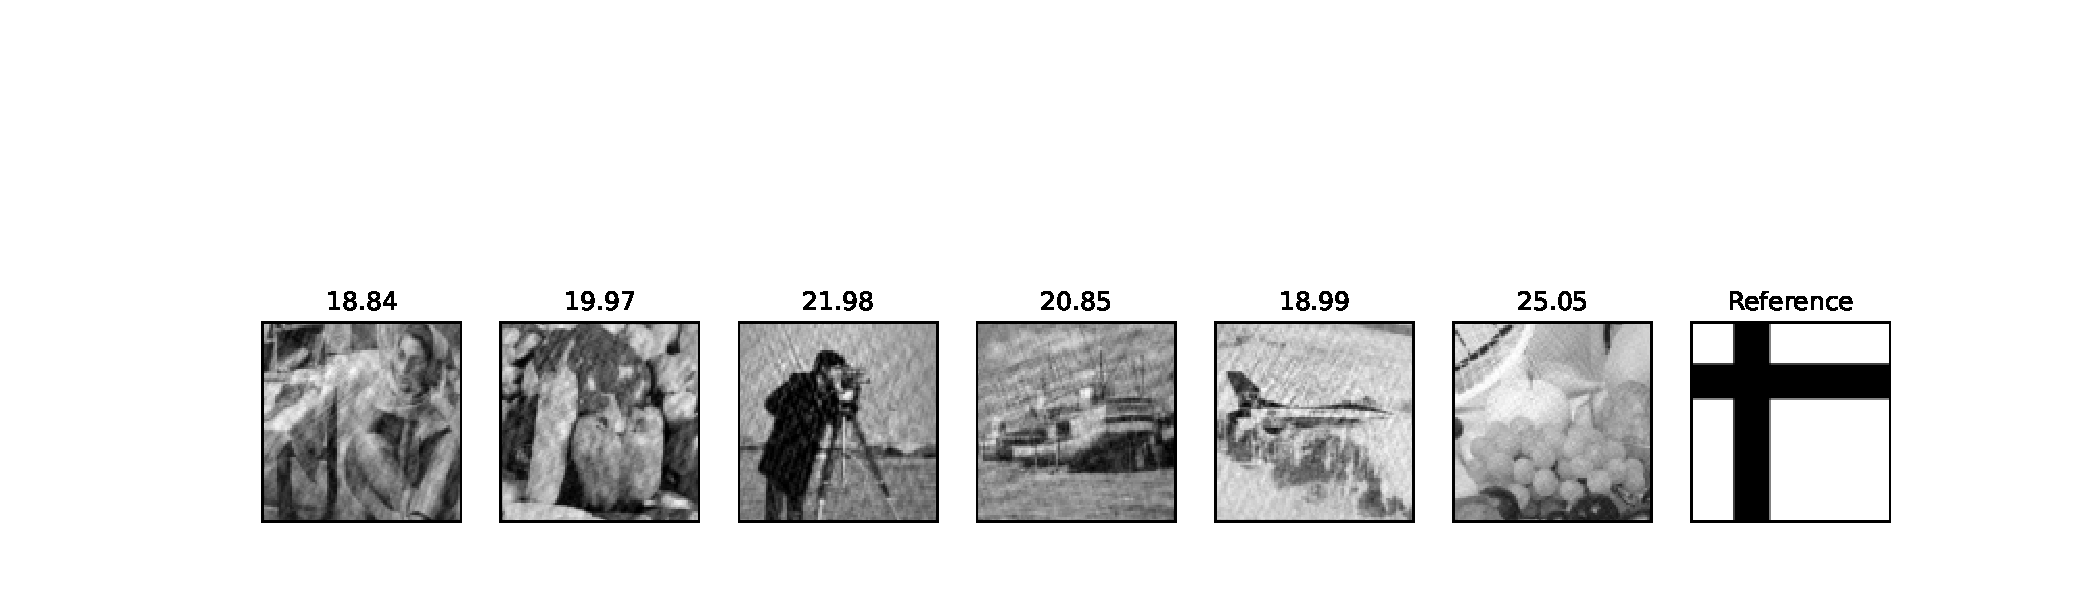
\includegraphics[trim=270 35 270 120, width=7.8cm]{data/rec-geometric-std.pdf}
		\caption{Reconstruction using a handcrafted reference }
	\end{subfigure}
	\caption{Reconstruction results on benchmark images using different references (PSNR on top). From top to bottom: ground truth, our trained CelebA reference, our trained CIFAR-10 reference,  best random reference (uniform distributed, evaluation on $100$ references per image), best handcrafted reference.}
	\label{images}
\end{figure}

\subsection{Comparison With Baseline Algorithm}

%Experiment~4.6 from~\cite{hyder2020solving} compares the proposed method to other phase retrieval methods and show that their approach performs best in comparison.
In this section, we validate the reported results of the hybrid-input-output algorithm (HIO)~\cite{Fienup:82} and extend the experimental evaluation by including two more baseline phase retrieval algorithms: Fienup's input-output and the Gerchberg-Saxton (GS) algorithm~\cite{Gerchberg1972APA}. We re-implement all three algorithms from scratch using NumPy~\cite{numpy}. We oversample the test images four times in spatial domain and run the algorithms for $100$ iterations on each image with a step size of $\beta=0.8$ for input-output~\cite{Fienup:82} and HIO~\cite{Fienup:82}. Also, the reconstructions are clipped to intensity values in range $[0, 1]$. For each image, we select the best PSNR from the cropped reconstruction and the cropped, flipped and shifted one. Tab.~\ref{results:baseline} shows the results on the different datasets. Overall, we can validate the claim by Hyder et al.~\cite{hyder2020solving}, even though our HIO~\cite{Fienup:82} implementation performs slightly better than the one reported in the original work.
\begin{landscape}
\begin{table*}
	\centering\small
	\begin{tabular}{llccccc}
		\toprule
		& Algorithm & MNIST& EMNIST& FMNIST & SVHN & CIFAR-10 \\
		\midrule

		\multirow{3}{*}{Ours} & Input-Output & $ \phantom{0}9.80\pm \phantom{0}1.35$ & $ \phantom{0}9.85\pm \phantom{0}1.46$ & $\phantom{0}8.74 \pm  \phantom{0}2.63$ & $\phantom{0}6.68 \pm \phantom{0}1.85$ & $\phantom{0}7.80 \pm \phantom{0}1.73$ \\

		& GS & $\phantom{0}9.82\pm \phantom{0}2.44$ & $ \phantom{0}9.99\pm \phantom{0}2.41$ & $11.25 \pm  \phantom{0}3.63$ & $17.89 \pm \phantom{0}3.77$ & $ 16.34\pm \phantom{0}3.08$ \\

		& HIO  & $10.53\pm \phantom{0}3.81 $& $10.81\pm \phantom{0}3.93$ & $14.06 \pm \phantom{0}8.54$ &  $31.90 \pm 16.45$ & $28.33 \pm 13.92$ \\
		\midrule
		\multirow{1}{*}{Hyder et al. \cite{hyder2020solving}} & HIO & $\phantom{0}9.04$ & $\phantom{0}8.42 $ & $\phantom{0}9.65$ & $19.87$ & $14.70$ \\
		\bottomrule
	\end{tabular}
	\caption{Comparison of mean PSNR values (with standard deviation) by the baseline methods without use of a reference signal. Additionally, to the results of the HIO algorithm, we report the results for the input-output and the GS algorithm.}
	\label{results:baseline}
\end{table*}
\end{landscape}

\subsection{Hyperparameter Search}
\label{sec:hyperp-search}
Since we have no access to the original learning rates, we perform an extensive
grid search on the hyperparameters $\alpha$ and $\beta$. In this study we use $5$ epochs during training and evaluate on $1000$ images.

We start with the learning rate $\alpha$ which is used to update the
reconstruction in training a reference and also in the retrieval
process. For this, we use the self-trained references and keep $\beta = 1$
fixed while $\alpha$ is variable in recovery. Our results on all used datasets are presented in
Fig.~\ref{hyperparam-all}.
Surprisingly, there is a general increase
of the mean PSNR among all datasets for rising $\alpha$ values up to a
peak in range $\alpha \in [1.75, 2.00]$. %Therefore, it is a property of the recovery process itself.
Unfortunately, also the standard deviation grows proportional to the higher mean PSNR
values. Nevertheless, these effects are stronger on artificial images
than on real-world images.

\begin{figure}
	\centering
	\includegraphics[width=7cm,trim= 10 20 10 0]{data/lr-alpha-rec-all.pdf}
	\caption{Results from the hyperparameter search for variable learning rate $\alpha$ in reconstruction.}
	\label{hyperparam-all}
\end{figure}

\begin{figure}
	\begin{subfigure}{.49\textwidth}
		\centering
		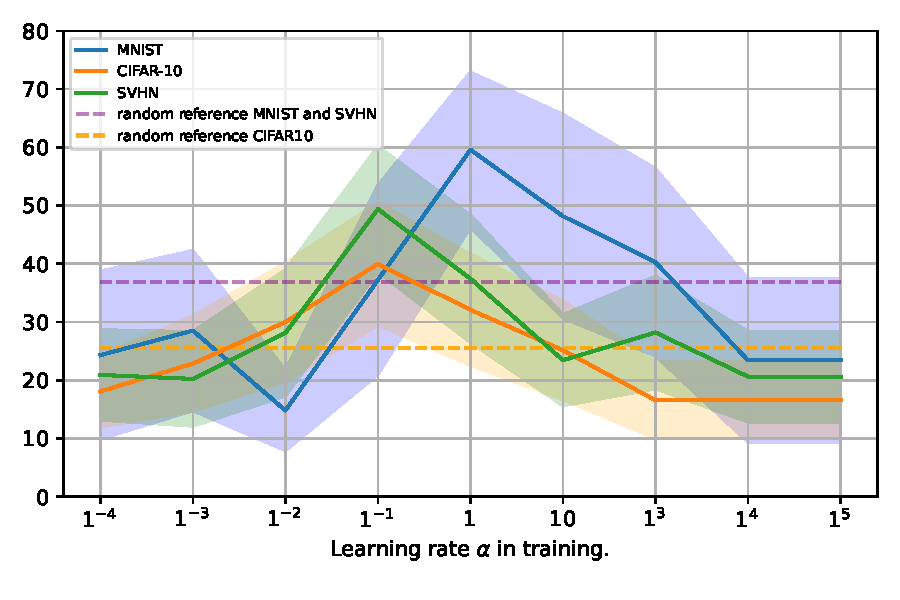
\includegraphics[width=6cm, trim= 0 20 0 0]{data/lr-alpha-log-plot-big.pdf}
		\caption{}
		\label{hyperparam-log-a}
	\end{subfigure}
	\begin{subfigure}{.49\textwidth}
		\centering
		\includegraphics[width=6cm, trim= 0 20 0 0]{data/lr-beta-log-plot-big.pdf}
		\caption{}
		\label{hyperparam-log-b}
	\end{subfigure}
	\caption{Results from the hyperparameter search for the learning rates: (a) mean PSNR of reconstructed images with  with references trained using different learning rates $\alpha$ and (b) mean PSNR of reconstructed images with references trained using different learning rates $\beta$. During reconstruction a fixed learning rate $\alpha=1$ has been used.}
\end{figure}

For our second experiment, we train with variable $\alpha$ on a logarithmic scale
while we keep $\beta=1$ fixed in training and fix $\alpha = 1$ in the
recovery process. Fig.~\ref{hyperparam-log-a} shows our results. Among
the considered datasets SVHN has the smallest range but provides still
valuable reconstructions for $\alpha \in [0.1, 1]$. However, for all
datasets, an extensively small or big $\alpha$ leads to learning a worse reference than a randomly sampled one, while the best recovery results are mainly in $\alpha \in [0.1, 1]$.

Finally, we train with a variable reference learning rate $\beta$, while we keep $\alpha=1$ fixed. Our results on a
representative subset are shown in Fig.~\ref{hyperparam-log-b}. In
general, choosing small value for $\beta$ leads to learning useless references. Nevertheless, we observe no general pattern for optimizing the retrieval performance by adjusting $\beta$ in training
but valuable results often ranges in the interval $\beta \in [0.1,10]$.


\subsection{Ablation Study}

\begin{figure}
	\begin{subfigure}{.24\textwidth}
		\centering
		\includegraphics[width=3cm, trim= 10 35 10 120]{data/zero-oversampling.pdf}
		\caption{No oversampling}
	\end{subfigure}
	\begin{subfigure}{.24\textwidth}
		\centering
		
\includegraphics[width=3cm, trim= 10 35 10 120]{data/two-times-oversampling.pdf}
		\caption{$2\times$ oversampling}
	\end{subfigure}
	\begin{subfigure}{.24\textwidth}
		\centering
		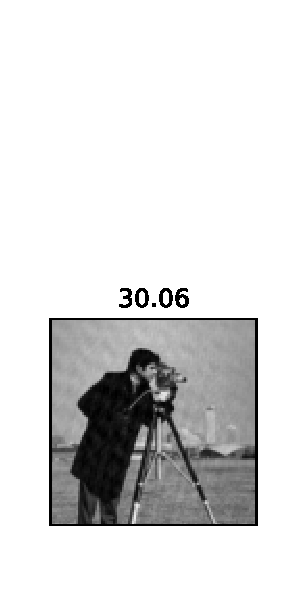
\includegraphics[width=3cm, trim= 10 35 10 120]{data/four-times-oversampling.pdf}
		\caption{$4\times$ oversampling}
	\end{subfigure}
	\begin{subfigure}{.24\textwidth}
		\centering
		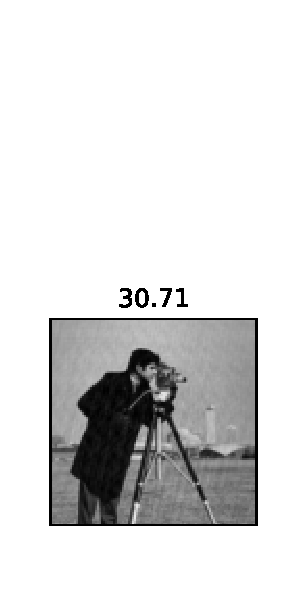
\includegraphics[width=3cm, trim= 10 35 10 120]{data/eight-times-oversampling.pdf}
		\caption{$8\times$ oversampling}
	\end{subfigure}
	\caption{Reconstructions results with CelebA reference (trained with oversampling) and use of different amount of oversampling during reconstruction (mean PSNR values on top of the images).}
	\label{oversampling}
\end{figure}

For our ablation study we investigate whether a reference is really
necessary for the retrieval process and study how oversampling
in spatial domain influences the reconstruction quality. For this
experiment, we use MNIST, CIFAR-10 with $1000$ test images as well as
the common ``cameraman'' image in shape $512 \times 512$. The learning rates are fixed to $\alpha=1$ and $\beta=1$.

First, we run the reconstruction algorithm without using a reference. We observe that the mean PSNR decreases drastically, e.g., for MNIST the mean PSNR is $8.92\text{dB}$. We observed similar results for other datasets such that we can conclude that a reference is required to obtain reasonable reconstructions.

Second, we use a reference that was trained with  $4\times$ oversampling and we vary the amount of oversampling during the recovery process. Fig.~\ref{oversampling} shows our results for a single benchmark image. We observe, that using no oversampling or $2\times$ oversampling during reconstruction leads to cloud-like artifacts. Oversampling $4\times$ in recovery is successful. Oversampling by a factor of $8$ leads only to marginally improved performance.

Additionally, we find that we can obtain reasonable reconstructions with references that were trained without any oversampling, if we use $4\times$  oversampling in the retrieval process. For example, using this approach we receive a mean PSNR of $47.90\text{dB}$ on MNIST which is just $6.38 \text{dB}$ PSNR below the result with a reference that was trained using $4 \times$ oversampling. Therefore, it might be a consideration to omit oversampling while training a reference, as it is a trade-off between reconstruction quality and computational requirements.



\section{Discussion}

%Give your judgement on if you feel the evidence you got from running the code supports the claims of the paper. Discuss the strengths and weaknesses of your approach - perhaps you didn't have time to run all the experiments, or perhaps you did additional experiments that further strengthened the claims in the paper.

In conclusion, we can verify that the unrolled network proposed by Hyder et al.~\cite{hyder2020solving} is capable of learning a valuable reference that can be utilized to recover a signal from its Fourier magnitude measurement. We trained our references from scratch and we demonstrated that they are similar enough to the original ones. Moreover, we encountered no major contradiction in our experiments if we use new data, references or generative methods.
However, an extensive hyperparameter search was necessary to match the reported results.  Also, the hyperparameter search reveals that one should focus on tuning the learning rate $\alpha$ during reconstruction as it yields to performance improvements across all datasets. Our ablation study shows that oversampling during training can be omitted to save computational resources.

Nonetheless, by providing an official implementation of their algorithm the authors enabled future researchers to utilize their method. Furthermore, we are grateful to the authors for kindly answering all of our questions regarding the implementation and providing feedback on our results.


%\bibliography{references}
%\bibliographystyle{plain}

